\documentclass[11pt,compress,t,notes=noshow, xcolor=table]{beamer}
\usepackage[]{graphicx}\usepackage[]{color}
% maxwidth is the original width if it is less than linewidth
% otherwise use linewidth (to make sure the graphics do not exceed the margin)
\makeatletter
\def\maxwidth{ %
  \ifdim\Gin@nat@width>\linewidth
    \linewidth
  \else
    \Gin@nat@width
  \fi
}
\makeatother

\definecolor{fgcolor}{rgb}{0.345, 0.345, 0.345}
\newcommand{\hlnum}[1]{\textcolor[rgb]{0.686,0.059,0.569}{#1}}%
\newcommand{\hlstr}[1]{\textcolor[rgb]{0.192,0.494,0.8}{#1}}%
\newcommand{\hlcom}[1]{\textcolor[rgb]{0.678,0.584,0.686}{\textit{#1}}}%
\newcommand{\hlopt}[1]{\textcolor[rgb]{0,0,0}{#1}}%
\newcommand{\hlstd}[1]{\textcolor[rgb]{0.345,0.345,0.345}{#1}}%
\newcommand{\hlkwa}[1]{\textcolor[rgb]{0.161,0.373,0.58}{\textbf{#1}}}%
\newcommand{\hlkwb}[1]{\textcolor[rgb]{0.69,0.353,0.396}{#1}}%
\newcommand{\hlkwc}[1]{\textcolor[rgb]{0.333,0.667,0.333}{#1}}%
\newcommand{\hlkwd}[1]{\textcolor[rgb]{0.737,0.353,0.396}{\textbf{#1}}}%
\let\hlipl\hlkwb

\usepackage{framed}
\makeatletter
\newenvironment{kframe}{%
 \def\at@end@of@kframe{}%
 \ifinner\ifhmode%
  \def\at@end@of@kframe{\end{minipage}}%
  \begin{minipage}{\columnwidth}%
 \fi\fi%
 \def\FrameCommand##1{\hskip\@totalleftmargin \hskip-\fboxsep
 \colorbox{shadecolor}{##1}\hskip-\fboxsep
     % There is no \\@totalrightmargin, so:
     \hskip-\linewidth \hskip-\@totalleftmargin \hskip\columnwidth}%
 \MakeFramed {\advance\hsize-\width
   \@totalleftmargin\z@ \linewidth\hsize
   \@setminipage}}%
 {\par\unskip\endMakeFramed%
 \at@end@of@kframe}
\makeatother

\definecolor{shadecolor}{rgb}{.97, .97, .97}
\definecolor{messagecolor}{rgb}{0, 0, 0}
\definecolor{warningcolor}{rgb}{1, 0, 1}
\definecolor{errorcolor}{rgb}{1, 0, 0}
\newenvironment{knitrout}{}{} % an empty environment to be redefined in TeX

\usepackage{alltt}
\newcommand{\SweaveOpts}[1]{}  % do not interfere with LaTeX
\newcommand{\SweaveInput}[1]{} % because they are not real TeX commands
\newcommand{\Sexpr}[1]{}       % will only be parsed by R
\newcommand{\xmark}{\ding{55}}%


\usepackage[english]{babel}
\usepackage[utf8]{inputenc}

\usepackage{dsfont}
\usepackage{verbatim}
\usepackage{amsmath}
\usepackage{amsfonts}
\usepackage{amssymb}
\usepackage{bm}
\usepackage{csquotes}
\usepackage{multirow}
\usepackage{longtable}
\usepackage{booktabs}
\usepackage{enumerate}
\usepackage[absolute,overlay]{textpos}
\usepackage{psfrag}
\usepackage{algorithm}
\usepackage{algpseudocode}
\usepackage{eqnarray}
\usepackage{arydshln}
\usepackage{tabularx}
\usepackage{placeins}
\usepackage{tikz}
\usepackage{setspace}
\usepackage{colortbl}
\usepackage{mathtools}
\usepackage{wrapfig}
\usepackage{bm}
\usepackage{amsmath}
\usepackage{pifont}
\usepackage{xcolor} %colored math symbols

\usetikzlibrary{shapes,arrows,automata,positioning,calc,chains,trees, shadows}
\tikzset{
  %Define standard arrow tip
  >=stealth',
  %Define style for boxes
  punkt/.style={
    rectangle,
    rounded corners,
    draw=black, very thick,
    text width=6.5em,
    minimum height=2em,
    text centered},
  % Define arrow style
  pil/.style={
    ->,
    thick,
    shorten <=2pt,
    shorten >=2pt,}
}

\usepackage{subfig}

% Defines macros and environments
\usepackage{../../style/lmu-lecture}


\let\code=\texttt
\let\proglang=\textsf

\setkeys{Gin}{width=0.9\textwidth}

\setbeamertemplate{frametitle}{\expandafter\uppercase\expandafter\insertframetitle}

\usepackage{bbm}
% basic latex stuff
\newcommand{\pkg}[1]{{\fontseries{b}\selectfont #1}} %fontstyle for R packages
\newcommand{\lz}{\vspace{0.5cm}} %vertical space
\newcommand{\dlz}{\vspace{1cm}} %double vertical space
\newcommand{\oneliner}[1] % Oneliner for important statements
{\begin{block}{}\begin{center}\begin{Large}#1\end{Large}\end{center}\end{block}}


%new environments
\newenvironment{vbframe}  %frame with breaks and verbatim
{
 \begin{frame}[containsverbatim,allowframebreaks]
}
{
\end{frame}
}

\newenvironment{vframe}  %frame with verbatim without breaks (to avoid numbering one slided frames)
{
 \begin{frame}[containsverbatim]
}
{
\end{frame}
}

\newenvironment{blocki}[1]   % itemize block
{
 \begin{block}{#1}\begin{itemize}
}
{
\end{itemize}\end{block}
}

\newenvironment{fragileframe}[2]{  %fragile frame with framebreaks
\begin{frame}[allowframebreaks, fragile, environment = fragileframe]
\frametitle{#1}
#2}
{\end{frame}}


\newcommand{\myframe}[2]{  %short for frame with framebreaks
\begin{frame}[allowframebreaks]
\frametitle{#1}
#2
\end{frame}}

\newcommand{\remark}[1]{
  \textbf{Remark:} #1
}


\newenvironment{deleteframe}
{
\begingroup
\usebackgroundtemplate{
\includegraphics[width=\paperwidth,height=\paperheight]{../style/color/red.png}}
 \begin{frame}
}
{
\end{frame}
\endgroup
}
\newenvironment{simplifyframe}
{
\begingroup
\usebackgroundtemplate{
\includegraphics[width=\paperwidth,height=\paperheight]{../style/color/yellow.png}}
 \begin{frame}
}
{
\end{frame}
\endgroup
}\newenvironment{draftframe}
{
\begingroup
\usebackgroundtemplate{
\includegraphics[width=\paperwidth,height=\paperheight]{../style/color/green.jpg}}
 \begin{frame}
}
{
\end{frame}
\endgroup
}
% https://tex.stackexchange.com/a/261480: textcolor that works in mathmode
\makeatletter
\renewcommand*{\@textcolor}[3]{%
  \protect\leavevmode
  \begingroup
    \color#1{#2}#3%
  \endgroup
}
\makeatother


\input{../../latex-math/basic-math}
\input{../../latex-math/basic-ml}
\input{../../latex-math/ml-nn}

\newcommand{\titlefigure}{figure_man/earlystop.png}
\newcommand{\learninggoals}{
  \item Know how early stopping works 
  \item Understand how early stopping acts as a regularizer
  \item Know early stopping imitates $L2$ regularization in some cases
}

\title{Deep Learning}
\date{}

\begin{document}

\lecturechapter{Early Stopping}
\lecture{I2DL}

\begin{vbframe}{Early Stopping}
  
  \begin{itemize}
    \item When training with an iterative optimizer such as SGD, it is commonly the case that, after a certain number of iterations, generalization error begins to increase even though training error continues to decrease.     
    \item \textbf{Early stopping} refers to stopping the algorithm early before the generalization error increases.
  \end{itemize}
  \begin{figure}
    \centering
      \scalebox{0.5}{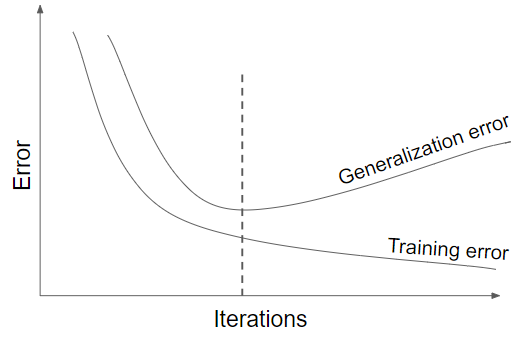
\includegraphics{figure_man/earlystop.png}}
      \caption{After a certain number of iterations, the algorithm begins to overfit.}
  \end{figure}
\framebreak
  How early stopping works:
  \begin{enumerate}
    \item Split training data $\Dtrain$ into $\mathcal{D}_{\text{subtrain}}$ and $\mathcal{D}_{\text{val}}$ (e.g. with a ratio of 2:1).
    \item Train on $\mathcal{D}_{\text{subtrain}}$ and evaluate model using the validation set $\mathcal{D}_{\text{val}}$.
    \item Stop training when validation error stops decreasing (after a range of \enquote{patience} steps).
    \item Use parameters of the previous step for the actual model.
  \end{enumerate}
  More sophisticated forms also apply cross-validation.
\end{vbframe}

\begin{vbframe}{Early Stopping and $L2$}
  \begin{table}
    \begin{tabular}{p{4cm}|p{6cm}}
    Strengths & Weaknesses \\
    \hline
    \hline
    Effective and simple & Periodical evaluation of validation error\\
    \hline
    Applicable to almost any model without adjustment \note{of objective function, parameter space, training procedure} & Temporary copy of $\thetav$ (we have to save the whole model each time validation error improves) \\
    \hline
    Combinable with other regularization methods & Less data for training $\rightarrow$ include $\mathcal{D}_{\text{val}}$ afterwards\\ \hline\hline
    \end{tabular}
  \end{table}
  \begin{itemize}
    \item For simple case of LM with squared loss and GD optim initialized at $\thetav=0$: Early stopping has exact correspondence with $L2$ regularization/WD: %Relation between
    optimal early-stopping iter $T_{\text{stop}}$ inversely proportional to  $\lambda$ scaled by step-size $\alpha$
    
 \end{itemize}
\begin{equation*}
T_{\text{stop}} \approx \frac{1}{\alpha \lambda} 
\Leftrightarrow \lambda \approx \frac{1}{T_{\text{stop}} \alpha}
\end{equation*}
  \begin{itemize}
    \item Small $\lambda$ ( regu. $\downarrow$) $\Rightarrow$ large $T_{\text{stop}}$ (complexity $\uparrow$) and vice versa
  \end{itemize}
\framebreak
  % \begin{itemize}
  %   \item[]
  % \end{itemize}
  % \begin{figure}
  %   \centering
  %     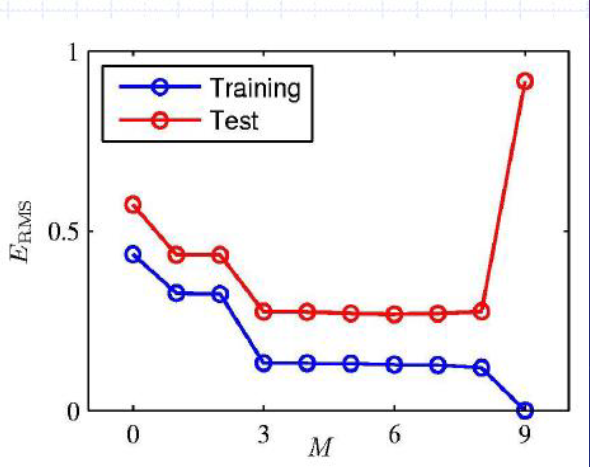
\includegraphics[width=11cm]{figure_man/early_stopping}
  %     \caption{Optimization path of early stopping (left) and weight decay (right) (Goodfellow et al. (2016))}
  % \end{figure}
  % \framebreak
  \begin{figure}
    \centering
      \scalebox{0.75}{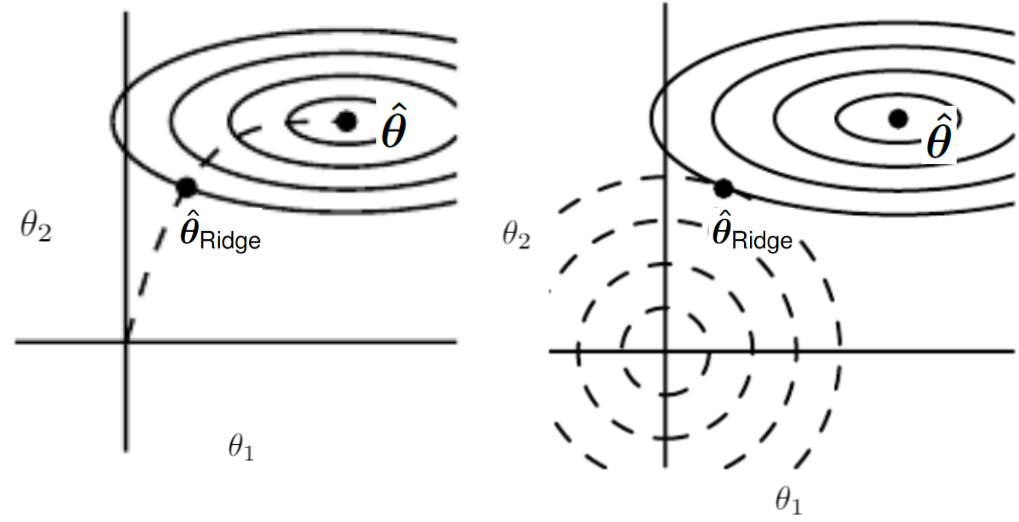
\includegraphics{figure_man/earlystop_int_hat.png}}
      \tiny{\\ \href{https://www.deeplearningbook.org/contents/regularization.html}{Goodfellow et al., 2016, p. 249 ff.}\\}
  \end{figure}
  
\footnotesize 
\textbf{Figure:} Effect of early stopping. \textit{Left:} The solid lines indicate contours of the square loss objective. Dashed line indicates trajectory taken by GD initialized at origin. Instead of reaching minimizer $\thetah$, ES results in trajectory stopping earlier at $\hat{\thetav}_{\text{ridge}}$. \textit{Right:} Effect of $L2$ regularization. Dashed circles indicate contours of $L2$ constraint which push minimizer of regularized cost closer to origin than minimizer of unregularized cost.
\end{vbframe}

\begin{vbframe}{SGD Trajectory and $L2$}
Solution paths for $L2$ regularized linear model closely matches SGD trajectory of unregularized LM initialized at $\thetav=0$
\lz
  \begin{figure}
    \centering
      %\scalebox{0.75}
      {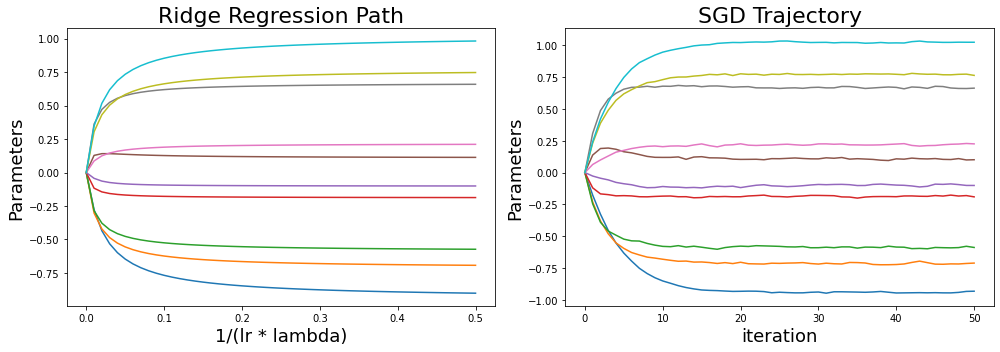
\includegraphics{figure_man/ridge-vs-sgd-path.png}}
      \scriptsize{\\ \href{https://proceedings.mlr.press/v119/ali20a/ali20a.pdf}{Ali et al., 2020}\\}
  \end{figure}

\textbf{Caveat}: Initialization at the origin is crucial for this equivalence to hold, which is almost never used in practice in ML/DL applications

\end{vbframe}

\endlecture
\end{document}
